\documentclass[12pt]{article} \usepackage{url, graphicx}

% page layout
\setlength{\topmargin}{-0.25in}
\setlength{\textheight}{9.5in}
\setlength{\headheight}{0in}
\setlength{\headsep}{0in}

% problem formatting
\newcommand{\problemname}{Problem}
\newcounter{problem}

% math
\newcommand{\dd}{\mathrm{d}}

% primary units
\newcommand{\rad}{\mathrm{rad}}
\newcommand{\kg}{\mathrm{kg}}
\newcommand{\m}{\mathrm{m}}
\newcommand{\s}{\mathrm{s}}

% secondary units
\renewcommand{\deg}{\mathrm{deg}}
\newcommand{\km}{\mathrm{km}}
\newcommand{\mi}{\mathrm{mi}}
\newcommand{\h}{\mathrm{h}}
\newcommand{\ns}{\mathrm{ns}}
\newcommand{\J}{\mathrm{J}}
\newcommand{\eV}{\mathrm{eV}}
\newcommand{\W}{\mathrm{W}}

% derived units
\newcommand{\mps}{\m\,\s^{-1}}
\newcommand{\mph}{\mi\,\h^{-1}}
\newcommand{\mpss}{\m\,\s^{-2}}

% random stuff
\sloppy\sloppypar\raggedbottom\frenchspacing\thispagestyle{empty}

\begin{document}

\noindent
Name: \rule[-1ex]{0.55\textwidth}{0.1pt}
NetID: \rule[-1ex]{0.2\textwidth}{0.1pt}

\section*{NYU Physics I---Term Exam 4}

\paragraph{\problemname~\theproblem:}\refstepcounter{problem}%
Roughly what is the quality factor $Q$ of this oscillator? (From
Lecture on 2016-10-25.) \\
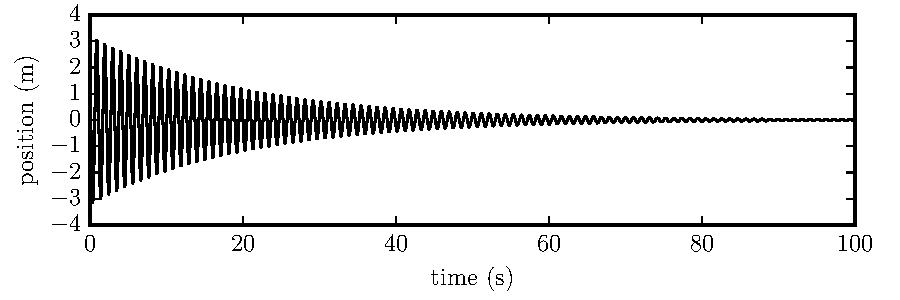
\includegraphics[width=0.66\textwidth]{../py/damped_oscillation.pdf}

\vfill

\paragraph{\problemname~\theproblem:}\refstepcounter{problem}%
Consider an ice cube that is $2\,\cm$ on a side, floating in water, in
normal New York circumstances. Roughly what is the atmospheric
pressure force (give a numerical answer in units of Newtons) acting on
the top face of this cube?  (From Lecture on 2016-11-01.)

\vfill

\paragraph{\problemname~\theproblem:}\refstepcounter{problem}%
A typical adult is holding her or his left arm at a right angle, so
the upper arm is pointing straight down, and the forearm is pointing
horizontally forwards.  The hand is oriented palm-up.  The arm is
holding a heavy grocery bag by its handle in the hand.  Draw a
free-body diagram for the hand-plus-forearm system, identifying all
significant forces acting on it. (From Problem Set 7.)

\vfill
~
\clearpage

\paragraph{\problemname~\theproblem:}\refstepcounter{problem}%
A modulus $E$ is a stress divided by a strain. What are the units of $E$?
(From Problem Set 8.)

\vfill

\paragraph{\problemname~\theproblem:}\refstepcounter{problem}%
A mass $M$ attached to a spring of spring constant $k$ is released
from rest a distance $X$ from its equilibrium position. It oscillates
with amplitude $X$. What is the maximum \emph{kinetic energy} $K_{\mathrm{max}}$ that
this mass ever attains in the future? Assume there is no damping and
it just oscillates. Give your answer in terms of $M$, $k$, and $X$ (or
any subset of these). (From the recitation on oscillations.)

\vfill

\paragraph{\problemname~\theproblem:}\refstepcounter{problem}%
If you have a potential of the form
$$
U(x) = A\,x^2 + B\,x + C
$$ where $A$ and $B$ are constants, where is the equilibrium position
$x_{\mathrm{eq}}$?  (From the recitation on potentials.)

\vfill
~
\end{document}
